\documentclass[text05.tex]{subfiles}
\begin{document}
\newpage
\section{\ruby{付録}{ふ|ろく}：センサー\ruby{紹介}{しょう|かい}}\label{sensor_intr}
\subsection{デジタル出力\ruby{装置}{そう|ち}}

\subsubsection{LED}\label{LED}
\begin{table}[H]
  \begin{widerrows} 
    \begin{tabular}{|p{\colF}|p{\colG}|}	\hline
    \ruby{名称}{めい|しょう} & LED（えるいーでぃー）\\ \hline
    \ruby{接続箇所}{せつ|ぞく|か|しょ} & デジタルコネクタ (3pin)\\ \hline
    \ruby{機能概要}{き|のう|がい|よう} & LEDを点灯させる\\ \hline
    \end{tabular}
  \end{widerrows} 
\end{table}

\begin{table}[H]
  \begin{widerrows} 
    \begin{tabular}{|p{\colF}|p{\colG}|}	\hline
    サンプルコードの場所 & 05/digout.hsp\\ \hline
    raspiへの入力 & なし\\ \hline
    raspiへの入力方法 & なし\\ \hline
    raspiからの出力 & \ruby{値}{あたい}が1の時点灯、\ruby{値}{あたい}が0の時消灯\\ \hline
    raspiからの出力方法 & gpio GPIO番号, パラメータ\\ \hline
    \end{tabular}
  \end{widerrows} 
\end{table}

\begin{table}[H]
  \begin{widerrows} 
    \begin{tabular}{|p{\colF}|p{\colG}|} \hline
    使い道 & 照明、信号機、車のライト\\ \hline
    \ruby{注意事項}{ちゅう|い|じ|こう} & なし\\ \hline
    \ruby{補足}{ほ|そく} & LEDチップの中で、マイナスの電気を持つ電子が、電子の\ruby{抜}{ぬ}けた\ruby{穴}{あな}である\ruby{正孔}{せい|こう}と結びつくと、エネルギーの一部が光になりま
  す。光の色は、使われている\ruby{半導体}{はん|どう|たい}の種類などによって決まります。\\ \hline
    \end{tabular}
  \end{widerrows} 
\end{table}

\begin{figure}[H]
  \begin{widerrows}
    \begin{tabular}{|p{\colH}|p{\colI}|p{\colH}|p{\colI}|} \hline
    外観 & 
    \begin{minipage}[t]{\linewidth}
      \smallskip
        \centering
        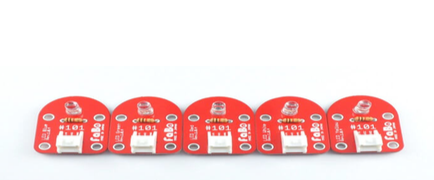
\includegraphics[width=0.8\linewidth]{../../asset/image/text05-img016.png}
        \caption{LED}
        \smallskip
      \end{minipage} &
      回路記号 & 
      \begin{minipage}[t]{\linewidth}
      \smallskip
        \centering
        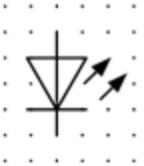
\includegraphics[width=0.3\linewidth]{../../asset/image/text05-img043.png}
        \caption{LEDの回路図}
        \smallskip
      \end{minipage}\\ \hline
    \end{tabular}
  \end{widerrows}
\end{figure}
\end{document}
